\section{Introduction}

This document describes the risk and opportunity management plan for the Vera C\. Rubin Observatory throughout operations.
The plan includes identifying, assessing, responding to, and managing risks and opportunities associated with the cost and schedule aspects.

The Rubin Observatory Risk \& Opportunity Board (RROB) serves as the managing group for the project.
The RROB is managed by the System Performance (SP) Department.

The model for managing risks and opportunities follows the NOIRLab model, see Figure \ref{fig:NOIRLab-risk-model}.
The project will use the Alcea Tracking Solutions (ATS) software tool, which is used and managed by NOIRLab for risk management of all its major projects.
The user guide for this tool is located on XXX.lsst.io --- the current draft is located at \url{https://docs.google.com/document/d/1Ep8FyDQO1jWnlKLvXxX_VfP-pPTrchssdxYOlgaaMrI/}.

\begin{figure}[t]
\caption{NOIRLab Risk Management Model.}
\centering
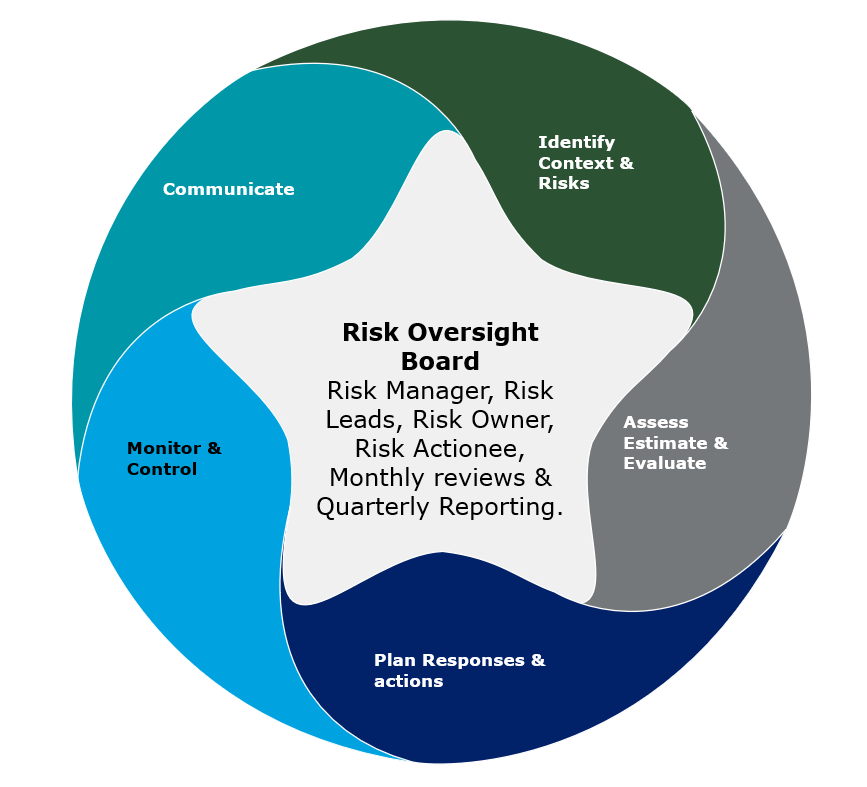
\includegraphics[width=\textwidth]{NOIRLab-risk-model-temp}
\label{fig:NOIRLab-risk-model}
\end{figure}

\subsection{Risk \& Opportunity Definitions}
\label{sec:definitions}

\textbf{Risk} (also known as \textbf{Threat}) ---
XXX.
Note that the term "risks" is used throughout this document as a negative impact, also known as a "threat" in the NOIRLab risk model.
Within the NOIRLab model, the term "risk" is used for positive (an "opportunity") and negative impacts.

\textbf{Existential Risk} --- 

\textbf{Opportunity} --- 

\textbf{Risk Responses} ---
The strategic process of controlling the identified risks, whereby the stakeholders decide how to deal with each risk and opportunities.

\textbf{Risk Actions} --- 
